
Se han seleccionado las siguientes tecnologías como alternativas de solución: Node.js con Express para el backend, React.js para el frontend, y MongoDB como base 
de datos. 

Estas decisiones conforman una arquitectura \textbf{MERN} (MongoDB, Express, React, Node.js), ejemplificada en la \coloredUnderline{\hyperlink{fig:arquitectura_mern}{Figura \ref*{fig:arquitectura_mern}: \nameref*{fig:arquitectura_mern}}}. 

Esta arquitectura presenta diversas ventajas, tales como la familiaridad de los desarrolladores con las tecnologías involucradas, el amplio soporte y documentación disponibles debido a su uso común en el desarrollo de aplicaciones web actuales,
y la facilidad de integración entre las tecnologías.

Se puede consultar más información sobre la arquitectura MERN en el siguiente enlace: \coloredUnderline{\href{https://www.mongodb.com/resources/languages/mern-stack}{MERN Stack}}.

\begin{figure}[H]
    \centering
    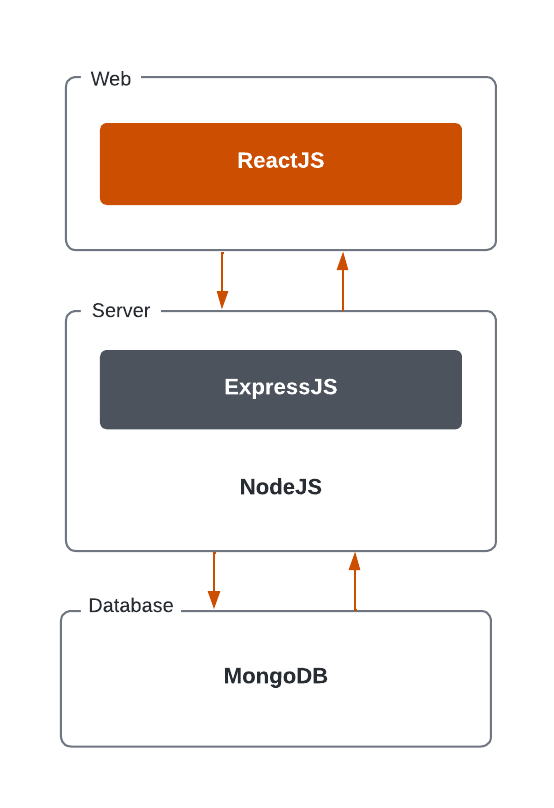
\includegraphics[width=0.4\textwidth]{figures/4-Estudio-viabilidad/4_MERN2.png}
    \caption{MERN Stack: MongoDB, Express, React, Node.js}
    \label{fig:arquitectura_mern}
    \hypertarget{fig:arquitectura_mern}{}
\end{figure}
